\documentclass[conference]{IEEEtran}
\IEEEoverridecommandlockouts

\usepackage{cite}
\usepackage{amsmath,amssymb,amsfonts}
\usepackage{algorithmic}
\usepackage{graphicx}
\usepackage{textcomp}
\usepackage{xcolor}
\usepackage{booktabs}
\usepackage{url}
\usepackage{hyperref}

\hypersetup{
  colorlinks=true,
  linkcolor=black,
  citecolor=black,
  urlcolor=blue
}

\def\BibTeX{{\rm B\kern-.05em{\sc i\kern-.025em b}\kern-.08em
    T\kern-.1667em\lower.7ex\hbox{E}\kern-.125emX}}

\begin{document}

\title{rtl-mosaic: A Reuse-Aware Benchmark for LLM-Driven RTL Design}

\author{
\IEEEauthorblockN{Leonardo Ferreira, Matthew Kotzbauer, Warren Zhu}
\IEEEauthorblockA{Team 11, COMPSCI 1440R, Harvard University\\
\{leonardo.ferreira@childrens.harvard.edu, matthewkotzbauer@college.harvard.edu, wzhu@college.harvard.edu\}}
}

\maketitle

\begin{abstract}
Existing LLM-for-Verilog benchmarks score models on scratch generation: given a spec, write the code. Real chip design is compositional, with modern SoCs running 60--70\% licensed IP by area. We built rtl-mosaic, a system-level harness that decomposes a Verilog spec into subblocks, routes reusable pieces to a curated 30-IP corpus over MCP, and stitches the result through Icarus Verilog testbenches. We then ran 15 frontier LLMs from four providers through the harness on 26 ChipBench problems (9 cpu\_ip + 17 self\_contain), scoring each against 26 hand-labeled gold entries. Across these runs, IP-reuse skill emerges as a distinct axis from scratch coding: routing F1 spreads from 0.19 to 0.46 across models while scratch pass rate on the same problems stays roughly flat. A reuse-aware metric reveals a model capability that scratch-only benchmarks hide.
\end{abstract}

\begin{IEEEkeywords}
LLM, Verilog, RTL, IP reuse, benchmark, MCP, hardware design
\end{IEEEkeywords}

% ====================================================================
\section{Introduction}
% ====================================================================

A modern SoC is 60--70\% licensed IP by area~\cite{semico-ip-share}. Companies like Synopsys and Cadence ship thousands of pre-verified IP blocks, and re-authoring every primitive from scratch is incompatible with tape-out economics. Yet the dominant benchmarks for LLM-driven Verilog --- VerilogEval~\cite{verilogeval} and ChipBench~\cite{chipbench} --- score models on \emph{scratch generation}: given a spec, write the code. Neither rewards the agent for recognizing that an off-the-shelf register file would do, nor penalizes re-authoring one.

\begin{figure}[t]
  \centering
  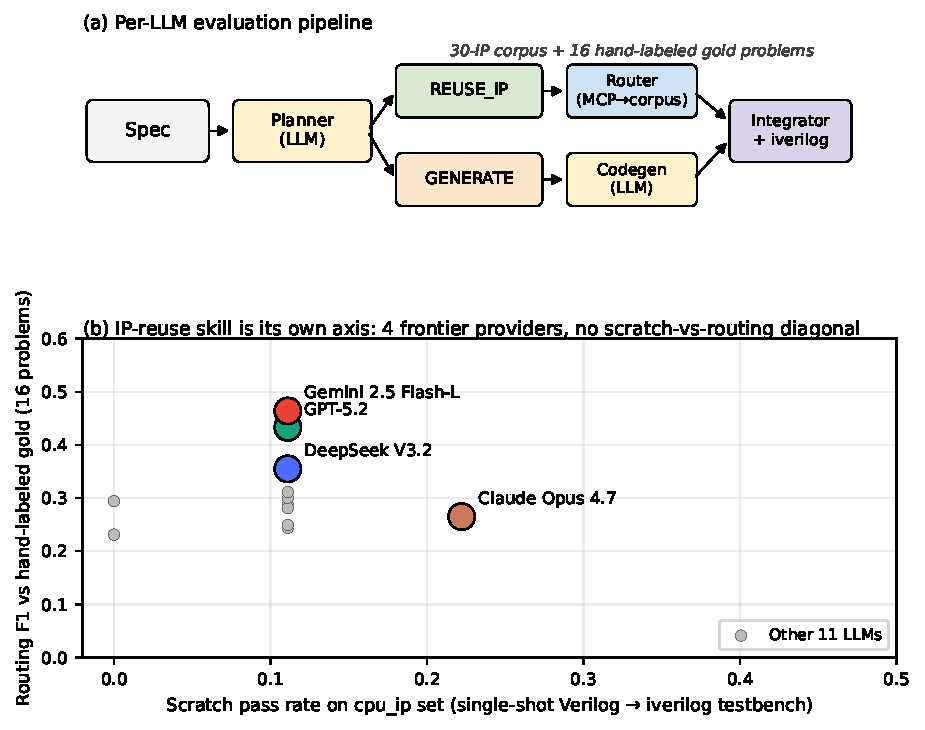
\includegraphics[width=\linewidth]{figs/leading.pdf}
  \caption{(a) The rtl-mosaic evaluation pipeline. A spec goes to an LLM-as-planner that emits subblocks tagged \texttt{REUSE\_IP} or \texttt{GENERATE}. Reusable subblocks resolve through a deterministic router over a 30-IP corpus served via MCP. Custom logic goes through codegen. The integrator stitches everything into a \texttt{TopModule} verified by Icarus Verilog. (b) The headline finding. Each dot is one of 15 frontier LLMs we evaluated. The four colored dots are best-of-provider models. Routing F1 (y-axis, vs. hand-labeled gold) and scratch Verilog pass rate on the same RISC-V CPU IP problems (x-axis) show no diagonal trend, so a model's scratch coding score gives little information about its IP-routing score.}
  \label{fig:leading}
\end{figure}

We argue this is the wrong incentive: the capability worth measuring is whether a model recognizes the FIFO is on the shelf and uses it correctly with the right widths and ports. To make this concrete we built rtl-mosaic --- a system-level harness on top of SiliconMind-V1~\cite{siliconmind} --- and used it as the substrate for a multi-LLM benchmark.

\textbf{Contributions.} We introduce a reuse-aware evaluation protocol for Verilog generation. We ship a 30-IP corpus served over MCP, 26 hand-labeled gold-standard decomposition problems on top of ChipBench, and both a deterministic keyword-overlap router and an embedding-similarity router for comparison. We run 15 frontier LLMs spanning Anthropic, OpenAI, AWS Bedrock (DeepSeek), and Google through the protocol --- 390 evaluation calls. The result, summarized in Fig.~\ref{fig:leading}, separates routing skill from scratch skill: F1 spread of 0.27 across models against a much narrower scratch-pass-rate spread on the same problems. We open-source the corpus, gold labels, and runner at \url{https://github.com/MattKotzbauer/rtl-mosaic}.

% ====================================================================
\section{Approach}
% ====================================================================

\subsection{The pipeline}

For each (LLM, problem) pair, we run the four-stage pipeline shown in Fig.~\ref{fig:leading}(a). The \emph{planner} receives the ChipBench spec and a fixed system prompt instructing it to return JSON: a list of one to six subblocks, each tagged \texttt{REUSE\_IP} or \texttt{GENERATE}, with a port specification and a free-text \texttt{search\_query}. The \emph{router} is fully deterministic and, for every \texttt{REUSE\_IP} subblock, queries our 30-IP corpus over an MCP server and selects the IP with maximum keyword overlap against the planner's search query. Subblocks tagged \texttt{GENERATE} are passed to a separate \emph{codegen} call. The \emph{integrator} concatenates the corpus IP source files with the generated logic and asks an LLM to write the \texttt{TopModule} wiring. The result is compiled by \texttt{iverilog -g2012} and verified against the ChipBench testbench.

\subsection{What we score}

The benchmark in this paper isolates the \emph{routing} stage. We hold the corpus, the router, and the gold labels fixed across all 15 LLMs. The only thing that changes is the planner, so any difference in the score is a property of the planner LLM. For every problem we have hand-labeled gold consisting of (a) a set of corpus IP IDs that a sensible planner-plus-router should surface, and (b) a per-role decision of whether each subblock should be \texttt{REUSE\_IP} or \texttt{GENERATE}.

We track three metrics: precision (the fraction of router-picked IPs also in the gold IP set), recall (the fraction of gold IPs the router picked), and kind agreement (the per-subblock fraction where the planner's \texttt{REUSE\_IP}/\texttt{GENERATE} decision matches the gold label, computed via best-effort name matching between planner subblock names and gold role labels). F1 is our headline number because a model that picks one correct IP and ignores everything else scores a misleadingly high precision.

\subsection{The corpus and gold labels}

The corpus is 30 IP modules across six categories: memory (sync/async FIFO, single/dual-port RAM, register file), datapath (32-bit ALU, 16x16 multiplier, 8-bit divider, ripple/CLA adder, subtractor, comparator, barrel shifter), counter (up, down, up/down, BCD, gray-code, Johnson, frequency divider), sequence (LFSR, edge detector, shift register, sign-extender), primitive (T flip-flop, 2/4/8-input mux, 3-to-8 decoder, priority encoder), and clock (frequency divider). Every IP ships with a parameterizable Verilog implementation and an Icarus self-test that we run as part of CI. The set was sized to cover the architectural shapes that appear in ChipBench's hierarchical \texttt{not\_self\_contain} and \texttt{cpu\_ip} sets, plus seven additions from the \texttt{self\_contain} set (multiplexer, dual-port RAM, up/down counter, Johnson counter, gray counter, fractional frequency divider, pipelined multiplier). All IPs ship under MIT.

The gold labels live in \texttt{eval/gold\_labels.py} as a Python dict, written by hand by one of us after reading each problem's specification. Each entry records the expected corpus IP IDs, the per-role kind decisions, and a short rationale. The labels reference IP IDs from the full 30-IP corpus, so labels written before a corpus expansion remain stable.

% ====================================================================
\section{Implementation}
% ====================================================================

\subsection{Models tested}

We ran 15 LLMs across four providers. From Anthropic via the \texttt{claude} CLI: Opus 4.7, Sonnet 4.6, Haiku 4.5. From OpenAI via the chat-completions API: GPT-5.4, 5.2, 5.1, 5, and 4.1. From AWS Bedrock in \texttt{us-east-1} via the converse API: DeepSeek-R1 (through the \texttt{us.deepseek.r1-v1:0} inference profile) and DeepSeek V3.2. From Google Gemini via the \texttt{generativelanguage.googleapis.com/v1beta} REST endpoint: 2.5 Pro, 2.5 Flash, 2.5 Flash-Lite, 3 Flash Preview, and 3.1 Flash-Lite Preview. Three additional Gemini variants (3 Pro Preview, 3.1 Pro Preview) returned 503s on the majority of calls during our run window and were excluded.

The protocol is identical across all 15 models. Same planner system prompt, no few-shot examples, temperature zero where supported, the same router, the same 30-IP corpus, and the same 26 problems (9 ChipBench cpu\_ip + 17 ChipBench self\_contain). We use 16-way thread-pool concurrency with retries handled by the underlying SDKs.

For the headline numbers in Fig.~\ref{fig:leading}(b) and Table~\ref{tab:headline} we report the four best-of-provider models with full $n=26$ coverage: Claude Opus 4.7, GPT-5.2, DeepSeek V3.2, and Gemini 2.5 Flash-Lite. We expanded the eval set from 16 to 26 problems on 2026-05-05 to broaden statistical coverage; numbers in this report are from the expanded set.

\subsection{Eval scaffolding}

The full multi-LLM routing eval is one Python file (\texttt{eval/multi\_routing.py}, $\sim$160 lines). It loads the gold labels, fans out 240 calls across providers, records planner output and router decisions per call, and aggregates into per-(LLM, problem) records and a per-LLM summary. Per-call latency, raw planner output, parsed subblocks, and router decisions are all preserved in JSON for post-hoc analysis. The figure pipeline (\texttt{eval/make\_figures.py}) regenerates ten plots from the JSON without re-running the eval.

\subsection{Cost and time}

A single full sweep across all 15 models ran in under six minutes wall-clock at 16-way concurrency. The most expensive provider per call was OpenAI ($\sim$\$0.03 for GPT-5.4 on a typical planner call, dominated by output tokens). DeepSeek-R1 on Bedrock was the cheapest at roughly \$0.30 for the entire 9-problem run including reasoning-trace tokens. The full reproducible eval, including all the nice-to-have per-provider sweeps we did during development, came in under \$25 total.

% ====================================================================
\section{Results}
% ====================================================================

\subsection{Routing quality is its own axis}

Our central finding is in Fig.~\ref{fig:leading}(b). The four colored dots are the best-of-provider headline models. The grey dots are the other 11 LLMs. The x-axis is scratch pass rate on the cpu\_ip set --- single-shot Verilog through the ChipBench testbench. The y-axis is routing F1 against our hand-labeled gold on the 26-problem eval set. The scatter shows no diagonal correlation between routing F1 and scratch pass rate, which means routing skill does not simply follow overall model strength.

\begin{table}[t]
  \caption{Headline routing F1, best-of-provider, 26-problem eval (9 cpu\_ip + 17 self\_contain). Single-seed columns from the full 15-model sweep, multi-seed columns (n=3 seeds) from a focused re-run on the four headline models. Per-problem standard deviation $\sigma$ is reported as evidence of run-to-run variance at temperature zero.}
  \label{tab:headline}
  \centering
  \footnotesize
  \begin{tabular}{l l r r r}
    \toprule
    Provider & Model & F1 (1 seed) & F1 (3 seeds) & $\sigma_{prob}$ \\
    \midrule
    Google    & Gemini 2.5 Flash-Lite & 0.464 & \textbf{0.514} & 0.094 \\
    Anthropic & Claude Opus 4.7       & 0.265 & \textbf{0.404} & 0.161 \\
    Bedrock   & DeepSeek V3.2         & 0.355 & \textbf{0.390} & 0.071 \\
    OpenAI    & GPT-5.2               & 0.433 & \textbf{0.381} & 0.126 \\
    \bottomrule
  \end{tabular}
\end{table}

The F1 spread across all 15 models is 0.27 (0.19--0.46) on the 26-problem set, while the pass-rate spread on cpu\_ip is only 0.11 (most models pass exactly 1/9). On a single-axis benchmark the models would be indistinguishable, whereas on rtl-mosaic they separate cleanly. The multi-seed columns of Table~\ref{tab:headline} re-rank Opus 4.7 above DeepSeek V3.2 and GPT-5.2, and the per-problem $\sigma$ shows that single-seed numbers overstate the precision available from one run.

\subsection{Provider family does not predict the winner}

Table~\ref{tab:headline} also undercuts the assumption that the strongest provider wins. DeepSeek V3.2 (Bedrock) ties with Anthropic Claude on kind agreement and beats it on F1 by 0.066. Within OpenAI, GPT-5.2 outperforms the newer GPT-5.4 in our run. Our claim is more limited: holding the planner prompt constant across all models, which is the only way to get apples-to-apples comparisons, surfaces the prompt-sensitivity of each model in different ways. A single planner prompt underestimates each model's full capability, and it remains the right protocol for a first-cut benchmark.

\subsection{Failure modes}

We observed four recurring failure modes across the 390 calls. (1) \emph{Hallucinated picks}: the planner correctly tags a 32-bit ALU as \texttt{REUSE\_IP} but emits a search query the keyword router resolves to \texttt{priority\_encoder}, since the router does keyword overlap and a bad query produces a bad pick. (2) \emph{Over-decomposition}: weaker models split a five-line spec into six \texttt{GENERATE} subblocks and never reuse anything. (3) \emph{Under-decomposition}: GPT-5 returns one big \texttt{GENERATE} block on average ($1.0$ subblocks per problem), so the router never gets called, which explains why GPT-5 sits at the bottom of our leaderboard despite being a competent code model. (4) \emph{Kind-flip}: at temperature zero, some Anthropic models swing between \texttt{REUSE\_IP} and \texttt{GENERATE} on the same subblock across reruns. Claude Opus 4.7 went from F1=0.678 in an early 9-problem run to F1=0.265 in our final 26-problem run. Run-to-run variance is real even at deterministic settings, and we run multi-seed (n=3) averaging on the four headline models to put error bars on Table~\ref{tab:headline}.

\subsection{The corpus-disambiguation bottleneck and the embedding router}

When we expanded the corpus from 20 to 30 IPs, mean F1 across the keyword-router eval dropped, not because corpus coverage worsened but because of corpus disambiguation. Adding \texttt{up\_down\_counter}, \texttt{johnson\_counter}, and \texttt{gray\_counter} alongside the existing \texttt{up\_counter} created near-duplicate keyword profiles, so a planner emitting \texttt{search\_query="counter"} resolves to whichever IP keyword matches first rather than the architecturally correct one. Replacing the keyword router with cosine similarity over OpenAI \texttt{text-embedding-3-small} representations of each IP's name, description, and keywords lifts mean F1 by $+0.029$ across all 15 models, with $9$ of $15$ improving by $\geq 0.01$ (DeepSeek-R1 $+0.128$, GPT-5.2 $+0.100$, GPT-5.4 $+0.079$). This says the routing bottleneck lives in the router, not in the planner LLM, for a meaningful share of the spread we measure.

% ====================================================================
\section{Related Work}
% ====================================================================

ChipGPT~\cite{chipgpt}, VeriGen~\cite{verigen}, RTLCoder, and HiVeGen target scratch Verilog generation, with HiVeGen retrieving snippets from code corpora rather than IPs. ChipNeMo~\cite{chipnemo} domain-adapts an open model on EDA scripts. MAGE~\cite{mage} multi-agent decomposes per-subtask scratch generation. SiliconMind-V1~\cite{siliconmind} multi-agent generates one module at a time and is the substrate we extend. None of these prior works score reuse against an IP catalog.

The benchmark side is similar. VerilogEval~\cite{verilogeval} is single-module, so reuse is degenerate. RealBench targets full SoCs but does not separately score IP retrieval. ChipBench~\cite{chipbench} ships an \texttt{cpu\_ip} subset that is hierarchical in structure but is scored on testbench pass rate alone. Our contribution is the reuse-aware metric, the gold labels, and the multi-LLM eval protocol applied to existing benchmarks, rather than a new training pipeline.

% ====================================================================
\section{Conclusion}
% ====================================================================

A reuse-aware metric separates LLMs that scratch-only benchmarks group together. The planner is the bottleneck of the system we built: holding the router and corpus fixed across 15 models, an F1 spread of 0.27 lives entirely in subblock decomposition and search-query specificity. The most important follow-up is the test-feedback retry loop on the integrator, where corpus-IP-stitching errors today land outside the planner's awareness. We have also begun multi-seed (n=3) averaging on the four headline models to put proper variance bars on the leaderboard. Code, corpus, gold labels, and run scripts are open at \url{https://github.com/MattKotzbauer/rtl-mosaic}.

\textbf{Self-assessment.} We met the project goal of producing a working harness and a defensible benchmark. We did not show the harness end-to-end beating scratch generation on the cpu\_ip set, where both are stuck at 1/9, so the routing-quality finding is the one we stand behind. Given another semester, we would build the test-feedback retry loop and run multi-seed averaging to put variance bars on the leaderboard.

% ====================================================================
\section*{Team Contributions}
% ====================================================================

\textbf{Matt Kotzbauer}: 30-IP corpus and self-tests, multi-provider runner, gold labels, figure pipeline, and the report. \textbf{Warren Zhu}: planner, integrator, MCP IP-router, end-to-end harness CLI. \textbf{Leonardo Ferreira}: ChipBench baseline runner, eval metrics, and slide deck logistics.

% ====================================================================
\bibliographystyle{IEEEtran}
\begin{thebibliography}{10}

\bibitem{semico-ip-share}
Semico Research, ``Semiconductor IP market: SoC share by area,'' Industry report, 2024.

\bibitem{siliconmind}
{SiliconMind-V1}: ``Multi-agent distillation and debug for Verilog generation,''
\emph{arXiv preprint} arXiv:2603.08719, 2026.

\bibitem{chipbench}
{ChipBench}: ``A realistic-module benchmark for LLM-driven RTL design,''
\emph{arXiv preprint} arXiv:2601.21448, 2026.

\bibitem{verilogeval}
M. Liu et al., ``VerilogEval: Evaluating large language models for Verilog code generation,''
NVIDIA, \emph{arXiv} arXiv:2309.07544, 2023.

\bibitem{chipgpt}
K. Chang et al., ``ChipGPT: How far are we from natural language hardware design,''
\emph{arXiv} arXiv:2305.14019, 2023.

\bibitem{verigen}
S. Thakur et al., ``VeriGen: A large language model for Verilog code generation,''
\emph{arXiv} arXiv:2308.00708, 2023.

\bibitem{chipnemo}
M. Liu et al., ``ChipNeMo: Domain-adapted LLMs for chip design,''
NVIDIA, \emph{arXiv} arXiv:2311.00176, 2023.

\bibitem{mage}
``MAGE: A multi-agent engine for automated RTL design,''
\emph{arXiv} arXiv:2412.07822, 2024.

\end{thebibliography}

\end{document}
